\chapter{Results: Sensitivity Analysis}
This chapter consists of the sensitivity analysis results of the 
EG01-30 \gls{NFC} transition scenario. 
Various types of \gls{SA} are conducted
using the Dakota-\Cyclus (\texttt{dcwrapper}) 
and Dakota-Dymond coupling (\texttt{ddwrapper}). 
This chapter will be broken into five sections: 
\begin{enumerate}
    \item Transition Scenario Specification 
    \item Sensitivity Analysis Evaluation Metrics 
    \item One-at-a-time \gls{SA} results 
    \item Synergistic \gls{SA} results
    \item Global \gls{SA} results 
\end{enumerate}

\section{Transition Scenario Specification}
% improve this section 
The same EG01-30 transition scenario is used for the Dymond 
sensitivity analysis and \Cyclus sensitivity analysis. 
The differences lie in the values of certain input variables but 
it is mostly the same. 

\subsection{Dymond}
Dymond transition scenario sensitivity analysis is conducted 
using the specifications of the Dymond OECD benchmark transition 
scenario presented at the 17th Meeting of Expert Group on Advanced 
Fuel Cycle Scenarios in France in 2017 
\cite{oecd_nuclear_energy_agency_wpfc_nodate}. 
The OECD benchmark scenario is based on the EG01-30 transition scenario in which 
the current \gls{PWR} fleet is transitioned to
a mixed fleet of \gls{MOX} \glspl{PWR} and \glspl{SFR}. 


\begin{table}[H]
    \caption{OECD Benchmark Transition Scenario
	Specifications \cite{oecd_nuclear_energy_agency_wpfc_nodate}}
	\label{tab:dymondinputs}
    \footnotesize
    \begin{tabularx}{\textwidth}{LL}
    \hline
                               \textbf{Input Parameter}            & \textbf{Value}            \\ \hline
    Demand driving commodity   & Power              \\
                               Demand equation {[}TWhe/y{]}   & 430        \\
                               Transition Start Date [Year] & 80\\ 
                               Fleet share ratio [\%] & \gls{MOX} \gls{PWR}: 15\%, \gls{SFR}: 85\%\\ \hline
    \end{tabularx}%
    \end{table}

\subsection{\Cyclus}
\Cyclus transition scenario sensitivity analysis will be conducted 
on the EG01-30 transition 
scenario for linearly increasing power demand (described in 
the section \ref{sec:eg01-30}). 
Figure \ref{fig:30flow} shows the facility and mass flow 
for this transition scenario in \Cyclus. 
Tables \ref{tab:bestinputs} and \ref{tab:facinputs}
shows the input parameters for \deploy and 
in the transition scenario. 
The \texttt{reactor} facility used in the \Cyclus simulation 
is a recipe reactor; it accepts a fresh fuel recipe and outputs 
a spent fuel recipe. 
The recipes used for the \gls{LWR}, \gls{MOX} \gls{LWR}, and 
\gls{SFR} are based on recipes generated by VISION 
\cite{chee_arfc/transition-scenarios_2018}
that closely match EG30 scenario specifications in 
Appendix B of the \gls{DOE} Evaluation and Screening Study 
(E\&S study) \cite{wigeland_nuclear_2014}. 
% describe input parameters and what was changed. 

\begin{table}[H]
    \caption{\Cyclus facility input parameters for
	EG01-EG30 transition scenario
	that minimizes undersupply for power and minimizes 
	the undersupply and under capacity for other facilities. }
	\label{tab:facinputs}
    \footnotesize
    \begin{tabularx}{\textwidth}{L|LL}
        \hline
        \textbf{Facility}                 & \textbf{Input Parameter}                    & \textbf{Value} \\ \hline
        \multirow{4}{*}{\textbf{LWR}}     & Lifetime {[}months{]}              & 960   \\
                                 & Cycle time {[}months{]}            & 18    \\
                                 & Refuel time {[}months{]}           & 1     \\
                                 & Rated Power {[}MWe{]}              & 1000  \\ \hline
        \multirow{2}{*}{\textbf{MOX LWR}} & Lifetime {[}months{]}              & 960   \\
                                 & Cycle time {[}months{]}            & 18    \\
                                 & Refuel time {[}months{]}           & 1     \\
                                 & Rated Power {[}MWe{]}              & 1000  \\ \hline
        \multirow{4}{*}{\textbf{SFR}}     & Lifetime {[}months{]}              & 720   \\
                                 & Cycle time {[}months{]}            & 12    \\
                                 & Refuel time {[}months{]}           & 1     \\
                                 & Rated Power {[}MWe{]}              & 333   \\ \hline
        \textbf{Cooling Pools}            & Used fuel storage time {[}years{]} & 3  \\ \hline
        \end{tabularx}
    \end{table}

\section{Sensitivity Analysis: Evaluation Metrics}
To determine the basis of comparison for sensitivity analysis 
of a \gls{NFC} transition scenario, important optimization 
metrics must be defined and associated with output variables.

In the E\&S study 
\cite{wigeland_nuclear_2014}, transition 
scenarios were evaluated for nine metrics: nuclear waste 
management, proliferation risk, nuclear material security risk, 
safety, environmental impact, resource utilization, development 
and deployment risk, institutional issues, financial risk and 
economics. 
These nine metrics can be further grouped and narrowed down to 
four categories \cite{passerini_systematic_2014}: environmental 
impact, economics, proliferation risk and resource utilization. 

To quantify the impact of the variation of an input parameter 
on an output parameter, it is necessary to define output indicators 
to measure this impact \cite{noauthor_effects_2017}. 
Output indicators are introduced because the output variables
are a time series resulting in a need for a single value that 
is representative of the output parameter's time series.  
Five types of output indicators are introduced 
\cite{noauthor_effects_2017}: 
(1) final value at end of simulation
(2) maximum value during simulation, 
(3) minimum value during simulation, 
(4) cumulative sum over the whole simulation, and 
(5) slope of the final 50 points of the simulation.
Depending on the nature of the output parameter, a different 
output indicator will be used. 
The slope indicator determines if a variable is increasing or 
decreasing at the end of the simulation. 
Indicators with transition refer to the indicator value during the 
transition period. 
The transition period is defined as from the year when the first 
transition reactor is built till the year of last idle capacity. 

Table \ref{tab:category-output-DD} shows the selected 
output variables used in this work and their associated 
evaluation metrics. 

% update for cyclus and dymond when decided
\begin{table}[H]
    \centering
    \caption {Evaluation metrics and their associated output 
    variables for sensitivity analysis.}
	\label{tab:category-output-DD}
        \footnotesize
        \begin{tabularx}{\textwidth}{l|LL}	
            	\hline
            \textbf{Evaluation Metrics} & \textbf{Output Variable} & \textbf{Indicators}\\
            \hline
            \textbf{Waste Management} & \begin{tabular}[c]{@{}l@{}}Total \gls{HLW} Inventory\\ Depleted Uranium\end{tabular} & \begin{tabular}[c]{@{}l@{}}Final \\ Final \end{tabular}\\
            \hline
            \textbf{Proliferation Risk} &  \begin{tabular}[c]{@{}l@{}}Pu in cooling pools\\ Separated Pu in storage \\ Separated Pu in HLW \\ 
            \end{tabular} & 
        \begin{tabular}[c]{@{}l@{}} Max, Quality\\ Max, Quality \\ Max, Quality \end{tabular} \\
            
            \hline
            \textbf{Resource Utilization} & Uranium ore consumed & Sum\\
            \hline
            \textbf{Goodness of Transition} & \begin{tabular}[c]{@{}l@{}}Total Idle Capacity\\ Date of Idle Capacity \\ Length of transition\end{tabular} & \begin{tabular}[c]{@{}l@{}}Sum \\ Final \\ -\end{tabular} \\ 
            \hline
            \end{tabularx}
\end{table}

The operational conditions for the advanced reactors and
the specifics of the transition scenario are not 
fixed since the fuel cycle simulator is modeling future 
trajectories. 
The input parameters that are varied in the
transition scenarios are: 
\begin{itemize}
    \item Length of cooling time for discharged fuel 
    \item Fleet share ratio of PWR MOX and SFR reactors 
	\item Introduction date of advanced reactor technology
\end{itemize}

The sensitivity analysis was conducted for both Dymond and \Cyclus. 

\section{One-at-a-time Sensitivity Analysis}

\subsection{Length of cooling time for discharged fuel}
Used fuel cooling time for all cooling pools was varied from 
0 to 8 years for the EG01-30 transition scenario. 
Each of these simulations are compared based on the evaluation 
metrics described in table \ref{tab:category-output-DD}.

\subsubsection{\textbf{Dymond}}
Table \ref{tab:dymond-ct} shows the absolute values of 
output variables associated with the environmental impact, 
resource utilization, and goodness of transition evaluation 
metrics for each scenario. 
Table \ref{tab:dymond-ct-sa} shows each scenario's percentage 
difference compared with the base case of `Cooling Time = 2 years'
scenario.

\begin{table}[H]
    \centering
    \caption{Dymond: Assessment of how variation of used fuel cooling times
    impacts evaluation metrics (waste management, resource utilization, 
    and goodness of transition) for OECD benchmark transition scenario.}
	\label{tab:dymond-ct-1}
        \footnotesize
        \begin{tabularx}{\textwidth}{L|LL|L|LLL}	
            \hline
            \textbf{} & \multicolumn{2}{c|}{\textbf{Environmental Impact}}                                                                                                                                                                                                                                                      & \textbf{Resource Utilization}                                                                                        & \multicolumn{3}{c}{\textbf{Goodness of Transition}}                                                                                                                                                                                 \\ \hline
\textbf{Scenario: Used Fuel Cooling Time} & \textbf{Final HLW [kg] } & \textbf{Final Depleted U [kg]} &  \textbf{Total U Ore [kg]}  & \textbf{Total Idle Capacity[kg]} & \textbf{Year of Final Idle Capacity} & \textbf{Length of Transition [years]} \\ \hline
 0  &           1103.2 &                             916933.4 &                       16188.8 &                                    30148.8 &                      301 &                     227 \\ 
 1  &           1101.6 &                             916618.2 &                       16188.8 &                                    30148.8 &                      301 &                     227 \\ 
 2  &           1105.7 &                             916237.60 &                       16188.8 &                                    30148.8 &                      301 &                     227 \\ 
 3  &           1108.3 &                             916268.7 &                       16188.8 &                                   256588.8 &                      301 &                     227 \\ 
 4  &           1099.8 &                             916962.4 &                       16188.8 &                                 1338604.8 &                      301 &                     227 \\ \hline
\end{tabularx}%
\end{table}

\begin{table}[H]
    \centering
    \caption{Dymond: Assessment of how variation of used fuel cooling times
    impacts evaluation metrics (proliferation risk) for OECD benchmark
	transition scenario.}
	\label{tab:dymond-ct-2}
        \footnotesize
        \begin{tabularx}{\textwidth}{L|LLLLLL}	
            \hline
            \textbf{} & \multicolumn{6}{c}{\textbf{Proliferation Risk}}  \\ \hline
\textbf{Scenario: Used Fuel Cooling Time} & \textbf{Max Pu in cooling pools [kg] } & \textbf{Pu Quality at max Pu in cooling pools [kg]} &  \textbf{Max Pu in HLW [kg]}  & \textbf{Pu Quality at max Pu in HLW [kg]} & \textbf{Max Pu in Rpr facilities [kg]} & \textbf{Pu Quality at max Pu in Rpr facilities [kg]} \\ \hline
 0  &           0.0 &                             0 &                       18.374 &                                    0.650 &                      208.6 &                     - \\ 
 1  &           105.2 &                             0.652 &                       18.385 &                                    0.652 &                      208.6 &                     - \\ 
 2  &           196.8 &                             0.622 &                       18.409 &                                    0.653 &                      208.6 &                     - \\ 
 3  &           264.8 &                             0.659 &                       18.189 &                                   0.654 &                      208.6 &                     - \\ 
 4  &           348.2 &                             0.671 &                       16.805 &                                 0.658 &                      208.6 &                     - \\ \hline
\end{tabularx}%
\end{table}

\begin{table}[H]
    \caption{Dymond: Sensitivity analysis of how variation of used fuel 
    cooling times impacts evaluation metrics (waste management, resource utilization, 
    and goodness of transition)for OECD benchmark transition scenario.
    The numbers in the table represent by how many \% an output variable 
    from each scenario differs from the base case.}
    \label{tab:dymond-ct-sa-1}
    \footnotesize
    \begin{tabularx}{\textwidth}{L|LL|L|LLL}	
		\hline
        \textbf{} & \multicolumn{2}{c|}{\textbf{Environmental Impact}}                                    & \textbf{Resource Utilization}                                                                                       & \multicolumn{3}{c}{\textbf{Goodness of Transition}}                                                                                                                                                                                 \\ \hline
        \textbf{Scenario: Used Fuel Cooling Time} & \textbf{Final HLW [kg] } & \textbf{Final Depleted U [kg]} &  \textbf{Total U Ore [kg]}  & \textbf{Total Idle Capacity[kg]} & \textbf{Year of Final Idle Capacity} & \textbf{Length of Transition [years]} \\ \hline
         0  &             \cellcolor[HTML]{67FD9A}-0.221736 &                                   \cellcolor[HTML]{67FD9A}0.075939 &                                                            \cellcolor[HTML]{67FD9A}0.0 &                 \cellcolor[HTML]{67FD9A}0.000000 &                                           \cellcolor[HTML]{67FD9A}0.0 & \cellcolor[HTML]{67FD9A}0.0 \\
		 1  &             \cellcolor[HTML]{67FD9A}-0.363540 &                                    \cellcolor[HTML]{67FD9A}0.041532 &                                                           \cellcolor[HTML]{67FD9A}0.0 &                 \cellcolor[HTML]{67FD9A}0.000000 &                                          \cellcolor[HTML]{67FD9A}0.0 & \cellcolor[HTML]{67FD9A}0.0 \\ 
		 2  &              \cellcolor[HTML]{000000}0.000000 &                                     \cellcolor[HTML]{000000}0.000000 &                                                              \cellcolor[HTML]{000000}0.0 &                 \cellcolor[HTML]{000000}0.000000 &                                         \cellcolor[HTML]{000000}0.0 & \cellcolor[HTML]{000000}0.0 \\ 
		 3  &              \cellcolor[HTML]{67FD9A}0.234524 &                                    \cellcolor[HTML]{67FD9A}0.003389 &                                                              \cellcolor[HTML]{67FD9A}0.0 &               \cellcolor[HTML]{FD6864}751.074670 &                                         \cellcolor[HTML]{67FD9A}0.0 & \cellcolor[HTML]{67FD9A}0.0 \\ 
		 4  &             \cellcolor[HTML]{67FD9A}-0.529033 &                                   \cellcolor[HTML]{67FD9A}0.079102 &                                                        \cellcolor[HTML]{67FD9A}0.0 &              \cellcolor[HTML]{FD6864}4339.993632 &                                        \cellcolor[HTML]{67FD9A}0.0 & \cellcolor[HTML]{67FD9A}0.0 \\ \hline
	\end{tabularx}%
    
    \resizebox{0.3\textwidth}{!}{
    \fbox{\begin{tabular}{ll}
        \textcolor{green}{$\blacksquare$} & $sensitivity \leq 1\%$ \\
        \textcolor{orange}{$\blacksquare$} & $1\% < sensitivity < 10\%$ \\
        \textcolor{red}{$\blacksquare$} & $sensitivity \geq 10\%$
        \end{tabular}}}
    \end{table}

    \begin{table}[H]
        \caption{Dymond: Sensitivity analysis of how variation of used fuel 
        cooling times impacts evaluation metrics (proliferation risk)for OECD benchmark transition scenario.
        The numbers in the table represent by how many \% an output variable 
        from each scenario differs from the base case.}
        \label{tab:dymond-ct-sa-2}
        \footnotesize
        \begin{tabularx}{\textwidth}{L|LLLLLL}	
            \hline
            \textbf{} & \multicolumn{6}{c}{\textbf{Proliferation Risk}}  \\ \hline
\textbf{Scenario: Used Fuel Cooling Time} & \textbf{Max Pu in cooling pools [kg] } & \textbf{Pu Quality at max Pu in cooling pools [kg]} &  \textbf{Max Pu in HLW [kg]}  & \textbf{Pu Quality at max Pu in HLW [kg]} & \textbf{Max Pu in Rpr facilities [kg]} & \textbf{Pu Quality at max Pu in Rpr facilities [kg]} \\ \hline
             0  &             \cellcolor[HTML]{FD6864}-100 &                                   \cellcolor[HTML]{FD6864}-100 &                                                            \cellcolor[HTML]{67FD9A}-0.19 &                 \cellcolor[HTML]{67FD9A}-0.459 &                                           \cellcolor[HTML]{67FD9A}0.0 & \cellcolor[HTML]{67FD9A}- \\
             1  &             \cellcolor[HTML]{FD6864}-46.5 &                                    \cellcolor[HTML]{FE996B}4.82 &                                                           \cellcolor[HTML]{67FD9A}-0.13 &                 \cellcolor[HTML]{67FD9A}-0.153 &                                          \cellcolor[HTML]{67FD9A}0.0 & \cellcolor[HTML]{67FD9A}- \\ 
             2  &              \cellcolor[HTML]{000000}0.000000 &                                     \cellcolor[HTML]{000000}0.000000 &                                                              \cellcolor[HTML]{000000}0.0 &                 \cellcolor[HTML]{000000}0.000000 &                                         \cellcolor[HTML]{000000}0.0 & \cellcolor[HTML]{000000}0.0 \\ 
             3  &              \cellcolor[HTML]{FD6864}34.5 &                                    \cellcolor[HTML]{FE996B}5.95 &                                                              \cellcolor[HTML]{FE996B}-1.20 &               \cellcolor[HTML]{FD6864}0.153 &                                         \cellcolor[HTML]{67FD9A}0.0 & \cellcolor[HTML]{67FD9A}- \\ 
             4  &             \cellcolor[HTML]{FD6864}76.9 &                                   \cellcolor[HTML]{FE996B}7.88 &                                                        \cellcolor[HTML]{FE996B}-8.71 &              \cellcolor[HTML]{FD6864}0.766 &                                        \cellcolor[HTML]{67FD9A}0.0 & \cellcolor[HTML]{67FD9A}- \\ \hline
        \end{tabularx}%
        
        \resizebox{0.3\textwidth}{!}{
        \fbox{\begin{tabular}{ll}
            \textcolor{green}{$\blacksquare$} & $sensitivity \leq 1\%$ \\
            \textcolor{orange}{$\blacksquare$} & $1\% < sensitivity < 10\%$ \\
            \textcolor{red}{$\blacksquare$} & $sensitivity \geq 10\%$
            \end{tabular}}}
        \end{table}

    
\subsubsection{\textbf{\Cyclus}}
\begin{table}[H]
    \centering
    \caption{\Cyclus: Assessment of how variation of used fuel cooling times
    impacts evaluation metrics for EG01-30 
	transition scenario.}
	\label{tab:cyclus-ct-1}
        \footnotesize
        \begin{tabularx}{\textwidth}{L|LL|L|LLL}
            \hline	
            \textbf{} & \multicolumn{2}{c|}{\textbf{Environmental Impact}}                                                                                                                                                                                                                                                      & \textbf{Resource Utilization}                                                                                        & \multicolumn{3}{c}{\textbf{Goodness of Transition}}                                                                                                                                                                                 \\ \hline
\textbf{Scenario: Used Fuel Cooling Time} & \textbf{Final HLW [kg] } & \textbf{Final Depleted U [kg]} &  \textbf{Total U Ore [kg]}  & \textbf{Total Idle Capacity[kg]} & \textbf{Year of Final Idle Capacity} & \textbf{Length of Transition [years]} \\ \hline

0  & 13223828.1 & 798818620.4      & 143700000000    & 135.1               & 962                     & 2                      \\
2  & 13073261.2 & 798818620.4      & 143700000000    & 135.1               & 962                     & 2                      \\
4  & 12906058.3 & 798818620.4      & 143700000000    & 135.1               & 962                     & 2                      \\
6  & 12795682.5 & 798818620.4      & 143700000000    & 135.1               & 962                     & 2                      \\
8  & 12726528.6 & 798818620.4      & 143700000000    & 135.1               & 962                     & 2                     \\ \hline 
        \end{tabularx}
\end{table}

\begin{table}[H]
    \centering
    \caption{\Cyclus: Assessment of how variation of used fuel cooling times
    impacts evaluation metrics (proliferation risk) for OECD benchmark
	transition scenario.}
	\label{tab:cyclus-ct-2}
        \footnotesize
        \begin{tabularx}{\textwidth}{L|LLLLLL}	
            \hline
            \textbf{} & \multicolumn{6}{c}{\textbf{Proliferation Risk}}  \\ \hline
\textbf{Scenario: Used Fuel Cooling Time} & \textbf{Max Pu in cooling pools [kg] } & \textbf{Pu Quality at max Pu in cooling pools [kg]} &  \textbf{Max Pu in HLW [kg]}  & \textbf{Pu Quality at max Pu in HLW [kg]} & \textbf{Max Pu in Rpr facilities [kg]} & \textbf{Pu Quality at max Pu in Rpr facilities [kg]} \\ \hline
 0  &           0.0 &                             0 &                       18.374 &                                    0.650 &                      208.6 &                     - \\ 
 1  &           105.2 &                             0.652 &                       18.385 &                                    0.652 &                      208.6 &                     - \\ 
 2  &           196.8 &                             0.622 &                       18.409 &                                    0.653 &                      208.6 &                     - \\ 
 3  &           264.8 &                             0.659 &                       18.189 &                                   0.654 &                      208.6 &                     - \\ 
 4  &           348.2 &                             0.671 &                       16.805 &                                 0.658 &                      208.6 &                     - \\ \hline
\end{tabularx}%
\end{table}

% add color 
\begin{table}[H]
    \caption{\Cyclus: Sensitivity Analysis Results for EG01-30
    transition scenario for different used fuel cooling times.
    The numbers in the table represent by how many \% an output variable 
    from each scenario differs from the base case.}
    \label{tab:cyclus-ct-sa-1}
    \footnotesize
    \begin{tabularx}{\textwidth}{L|LL|L|LLL}	
		\hline
        \textbf{} & \multicolumn{2}{c|}{\textbf{Environmental Impact}}                                    & \textbf{Resource Utilization}                                                                                       & \multicolumn{3}{c}{\textbf{Goodness of Transition}}                                                                                                                                                                                 \\ \hline
        \textbf{Scenario: Used Fuel Cooling Time} & \textbf{Final HLW [kg] } & \textbf{Final Depleted U [kg]} &  \textbf{Total U Ore [kg]}  & \textbf{Total Idle Capacity[kg]} & \textbf{Year of Final Idle Capacity} & \textbf{Length of Transition [years]} \\ \hline
        0  & \cellcolor[HTML]{FE996B}1.15      & \cellcolor[HTML]{67FD9A}0.0              & \cellcolor[HTML]{67FD9A}0.0               & \cellcolor[HTML]{67FD9A}0.0                 & \cellcolor[HTML]{67FD9A}0.0                     & \cellcolor[HTML]{67FD9A}0.0                    \\
        2  & \cellcolor[HTML]{000000}0.0       & \cellcolor[HTML]{000000}0.0              & \cellcolor[HTML]{000000}0.0               & \cellcolor[HTML]{000000}0.0                 & \cellcolor[HTML]{000000}0.0                     & \cellcolor[HTML]{000000}0.0                    \\
        4  & \cellcolor[HTML]{FE996B}-1.28       & \cellcolor[HTML]{67FD9A}0.0              & \cellcolor[HTML]{67FD9A}0.0               & \cellcolor[HTML]{67FD9A}0.0                 & \cellcolor[HTML]{67FD9A}0.0                     & \cellcolor[HTML]{67FD9A}0.0                    \\
        6  & \cellcolor[HTML]{67FD9A}-2.12     & \cellcolor[HTML]{67FD9A}0.0              & \cellcolor[HTML]{67FD9A}0.0               & \cellcolor[HTML]{67FD9A}0.0                 & \cellcolor[HTML]{67FD9A}0.0                     & \cellcolor[HTML]{67FD9A}0.0                    \\
        8  & \cellcolor[HTML]{FE996B}-2.65     & \cellcolor[HTML]{67FD9A}0.0              & \cellcolor[HTML]{67FD9A}0.0               & \cellcolor[HTML]{67FD9A}0.0                 & \cellcolor[HTML]{67FD9A}0.0                     & \cellcolor[HTML]{67FD9A}0.0                   \\ \hline 
                \end{tabularx}%
    
    \resizebox{0.3\textwidth}{!}{
    \fbox{\begin{tabular}{ll}
        \textcolor{green}{$\blacksquare$} & $sensitivity \leq 1\%$ \\
        \textcolor{orange}{$\blacksquare$} & $1\% < sensitivity < 10\%$ \\
        \textcolor{red}{$\blacksquare$} & $sensitivity \geq 10\%$
        \end{tabular}}}
    \end{table}

    \begin{table}[H]
        \caption{\Cyclus: Sensitivity analysis of how variation of used fuel 
        cooling times impacts evaluation metrics (proliferation risk)for OECD benchmark transition scenario.
        The numbers in the table represent by how many \% an output variable 
        from each scenario differs from the base case.}
        \label{tab:cyclus-ct-sa-2}
        \footnotesize
        \begin{tabularx}{\textwidth}{L|LLLLLL}	
            \hline
            \textbf{} & \multicolumn{6}{c}{\textbf{Proliferation Risk}}  \\ \hline
\textbf{Scenario: Used Fuel Cooling Time} & \textbf{Max Pu in cooling pools [kg] } & \textbf{Pu Quality at max Pu in cooling pools [kg]} &  \textbf{Max Pu in HLW [kg]}  & \textbf{Pu Quality at max Pu in HLW [kg]} & \textbf{Max Pu in Rpr facilities [kg]} & \textbf{Pu Quality at max Pu in Rpr facilities [kg]} \\ \hline
             0  &             \cellcolor[HTML]{FD6864}-100 &                                   \cellcolor[HTML]{FD6864}-100 &                                                            \cellcolor[HTML]{67FD9A}-0.19 &                 \cellcolor[HTML]{67FD9A}-0.459 &                                           \cellcolor[HTML]{67FD9A}0.0 & \cellcolor[HTML]{67FD9A}- \\
             1  &             \cellcolor[HTML]{FD6864}-46.5 &                                    \cellcolor[HTML]{FE996B}4.82 &                                                           \cellcolor[HTML]{67FD9A}-0.13 &                 \cellcolor[HTML]{67FD9A}-0.153 &                                          \cellcolor[HTML]{67FD9A}0.0 & \cellcolor[HTML]{67FD9A}- \\ 
             2  &              \cellcolor[HTML]{000000}0.000000 &                                     \cellcolor[HTML]{000000}0.000000 &                                                              \cellcolor[HTML]{000000}0.0 &                 \cellcolor[HTML]{000000}0.000000 &                                         \cellcolor[HTML]{000000}0.0 & \cellcolor[HTML]{000000}0.0 \\ 
             3  &              \cellcolor[HTML]{FD6864}34.5 &                                    \cellcolor[HTML]{FE996B}5.95 &                                                              \cellcolor[HTML]{FE996B}-1.20 &               \cellcolor[HTML]{FD6864}0.153 &                                         \cellcolor[HTML]{67FD9A}0.0 & \cellcolor[HTML]{67FD9A}- \\ 
             4  &             \cellcolor[HTML]{FD6864}76.9 &                                   \cellcolor[HTML]{FE996B}7.88 &                                                        \cellcolor[HTML]{FE996B}-8.71 &              \cellcolor[HTML]{FD6864}0.766 &                                        \cellcolor[HTML]{67FD9A}0.0 & \cellcolor[HTML]{67FD9A}- \\ \hline
        \end{tabularx}%
        
        \resizebox{0.3\textwidth}{!}{
        \fbox{\begin{tabular}{ll}
            \textcolor{green}{$\blacksquare$} & $sensitivity \leq 1\%$ \\
            \textcolor{orange}{$\blacksquare$} & $1\% < sensitivity < 10\%$ \\
            \textcolor{red}{$\blacksquare$} & $sensitivity \geq 10\%$
            \end{tabular}}}
        \end{table}

\subsection{Fleet share ratio of PWR MOX and SFR reactors}
\subsubsection{\textbf{\Cyclus}}
\begin{table}[H]
    \centering
    \caption{\Cyclus: Assessment of how variation of fleet share ratio
    of PWR MOX and SFR reactors
    impacts evaluation metrics for EG01-30 transition scenario.}
	\label{tab:cyclus-fs-1}
        \footnotesize
        \begin{tabularx}{\textwidth}{L|LL|L|LLL}
            \hline	
            \textbf{} & \multicolumn{2}{c|}{\textbf{Environmental Impact}}                                                                                                                                                                                                                                                      & \textbf{Resource Utilization}                                                                                        & \multicolumn{3}{c}{\textbf{Goodness of Transition}}                                                                                                                                                                                 \\ \hline
\textbf{Scenario: PWR MOX Fleet Share [\%]} & \textbf{Final HLW [kg] } & \textbf{Final Depleted U [kg]} &  \textbf{Total U Ore [kg]}  & \textbf{Total Idle Capacity[kg]} & \textbf{Year of Final Idle Capacity} & \textbf{Length of Transition [years]} \\ \hline

960  & 12959554.6 & 798818620.4      & 143700000000.0    & 135.1               & 962                     & 2                      \\
972  & 13069177.0 & 798818620.4      & 143700000000.0    & 120.9               & 972                     & 0                      \\
984  & 13220184.0 & 803332630.7      & 143700000000.0    & 121.1               & 980                     & 0                      \\
996  & 13360033.7 & 807846641.1      & 143700000000.0    & 121.1               & 980                     & 0                      \\
1008 & 13337086.8 & 807846641.1      & 143700000000.0    & 121.1               & 980                     & 0                     \\ \hline
        \end{tabularx}
\end{table}

\begin{table}[H]
    \caption{\Cyclus: Sensitivity Analysis Results for EG01-30
    transition scenario for different fleet share ratios.
    The numbers in the table represent by how many \% an output variable 
    from each scenario differs from the base case.}
    \label{tab:cyclus-fs-sa-1}
    \footnotesize
    \begin{tabularx}{\textwidth}{L|LL|L|LLL}	
		\hline
        \textbf{} & \multicolumn{2}{c|}{\textbf{Environmental Impact}}                                    & \textbf{Resource Utilization}                                                                                       & \multicolumn{3}{c}{\textbf{Goodness of Transition}}                                                                                                                                                                                 \\ \hline
        \textbf{Scenario: Used Fuel Cooling Time} & \textbf{Final HLW [kg] } & \textbf{Final Depleted U [kg]} &  \textbf{Total U Ore [kg]}  & \textbf{Total Idle Capacity[kg]} & \textbf{Year of Final Idle Capacity} & \textbf{Length of Transition [years]} \\ \hline
        0  & \cellcolor[HTML]{FE996B}1.49      & \cellcolor[HTML]{67FD9A}0.0              & \cellcolor[HTML]{67FD9A}0.0               & \cellcolor[HTML]{67FD9A}0.0                 & \cellcolor[HTML]{67FD9A}0.0                     & \cellcolor[HTML]{67FD9A}0.0                    \\
        5  & \cellcolor[HTML]{67FD9A}0.75      & \cellcolor[HTML]{67FD9A}0.0              & \cellcolor[HTML]{67FD9A}0.0               & \cellcolor[HTML]{67FD9A}0.0                 & \cellcolor[HTML]{67FD9A}0.0                     & \cellcolor[HTML]{67FD9A}0.0                    \\
        10 & \cellcolor[HTML]{67FD9A}0.71      & \cellcolor[HTML]{67FD9A}0.0              & \cellcolor[HTML]{67FD9A}0.0               & \cellcolor[HTML]{67FD9A}0.0                 & \cellcolor[HTML]{67FD9A}0.0                     & \cellcolor[HTML]{67FD9A}0.0                    \\
        15 & \cellcolor[HTML]{000000}0.0       & \cellcolor[HTML]{000000}0.0              & \cellcolor[HTML]{000000}0.0               & \cellcolor[HTML]{000000}0.0                 & \cellcolor[HTML]{000000}0.0                     & \cellcolor[HTML]{000000}0.0                    \\
        20 & \cellcolor[HTML]{67FD9A}0.33      & \cellcolor[HTML]{67FD9A}0.0              & \cellcolor[HTML]{67FD9A}0.0               & \cellcolor[HTML]{67FD9A}0.0                 & \cellcolor[HTML]{67FD9A}0.0                     & \cellcolor[HTML]{67FD9A}0.0                   \\ \hline
                       \end{tabularx}%
    
    \resizebox{0.3\textwidth}{!}{
    \fbox{\begin{tabular}{ll}
        \textcolor{green}{$\blacksquare$} & $sensitivity \leq 1\%$ \\
        \textcolor{orange}{$\blacksquare$} & $1\% < sensitivity < 10\%$ \\
        \textcolor{red}{$\blacksquare$} & $sensitivity \geq 10\%$
        \end{tabular}}}
    \end{table}


\subsection{Introduction date of advanced reactor technology}

\subsubsection{\textbf{\Cyclus}}
\begin{table}[H]
    \centering
    \caption{\Cyclus: Assessment of how variation of introduction date of 
    advanced reactor technology
    impacts evaluation metrics for EG01-30 transition scenario.}
	\label{tab:ty}
        \footnotesize
        \begin{tabularx}{\textwidth}{L|LL|L|LLL}
            \hline	
            \textbf{} & \multicolumn{2}{c|}{\textbf{Environmental Impact}}                                                                                                                                                                                                                                                      & \textbf{Resource Utilization}                                                                                        & \multicolumn{3}{c}{\textbf{Goodness of Transition}}                                                                                                                                                                                 \\ \hline
\textbf{Scenario: Intro date of advanced tech [Month]} & \textbf{Final HLW [kg] } & \textbf{Final Depleted U [kg]} &  \textbf{Total U Ore [kg]}  & \textbf{Total Idle Capacity[kg]} & \textbf{Year of Final Idle Capacity} & \textbf{Length of Transition [years]} \\ \hline

80  & 12959554.6 & 798818620.4      & 143700000000    & 135.1               & 962                     & 2                      \\
81  & 13069177.0 & 798818620.4      & 143700000000    & 120.9               & 972                     & 0                      \\
82  & 13220184.0 & 803332630.7      & 143700000000    & 121.1               & 980                     & 0                      \\
83  & 13360033.7 & 807846641.1      & 143700000000    & 121.1               & 980                     & 0                      \\
84 & 13337086.8 & 807846641.1      & 143700000000    & 121.1               & 980                     & 0                     \\ \hline
        \end{tabularx}
\end{table}

\begin{table}[H]
    \caption{\Cyclus: Sensitivity Analysis Results for EG01-30
    transition scenario with different used fuel cooling times.
    The numbers in the table represent by how many \% an output variable 
    from each scenario differs from the base case.}
    \label{tab:ty-sa}
    \footnotesize
    \begin{tabularx}{\textwidth}{L|LL|L|LLL}	
		\hline
        \textbf{} & \multicolumn{2}{c|}{\textbf{Environmental Impact}}                                    & \textbf{Resource Utilization}                                                                                       & \multicolumn{3}{c}{\textbf{Goodness of Transition}}                                                                                                                                                                                 \\ \hline
        \textbf{Scenario: Used Fuel Cooling Time} & \textbf{Final HLW [kg] } & \textbf{Final Depleted U [kg]} &  \textbf{Total U Ore [kg]}  & \textbf{Total Idle Capacity[kg]} & \textbf{Year of Final Idle Capacity} & \textbf{Length of Transition [years]} \\ \hline
        80  & \cellcolor[HTML]{000000}0.0       & \cellcolor[HTML]{000000}0.0              & \cellcolor[HTML]{000000}0.0               & \cellcolor[HTML]{000000}0.0                 & \cellcolor[HTML]{000000}0.0                     & \cellcolor[HTML]{000000}0.0                    \\
        81  & \cellcolor[HTML]{67FD9A}0.85      & \cellcolor[HTML]{67FD9A}0.0              & \cellcolor[HTML]{67FD9A}0.0               & \cellcolor[HTML]{FD6864}-10.51              & \cellcolor[HTML]{FE996B}1.04                    & \cellcolor[HTML]{FD6864}-100.0                 \\
        82  & \cellcolor[HTML]{FE996B}2.01      & \cellcolor[HTML]{67FD9A}0.57             & \cellcolor[HTML]{67FD9A}0.0               & \cellcolor[HTML]{FD6864}-10.36              & \cellcolor[HTML]{FE996B}1.87                    & \cellcolor[HTML]{FD6864}-100.0                 \\
        83  & \cellcolor[HTML]{FE996B}3.09      & \cellcolor[HTML]{FE996B}1.13             & \cellcolor[HTML]{67FD9A}0.0               & \cellcolor[HTML]{FD6864}-10.36              & \cellcolor[HTML]{FE996B}1.87                    & \cellcolor[HTML]{FD6864}-100.0                 \\
        84 & \cellcolor[HTML]{FE996B}2.91      & \cellcolor[HTML]{FE996B}1.13             & \cellcolor[HTML]{67FD9A}0.0               & \cellcolor[HTML]{FD6864}-10.36              & \cellcolor[HTML]{FE996B}1.87                    & \cellcolor[HTML]{FD6864}-100.0                \\ \hline
                   \end{tabularx}%
    
    \resizebox{0.3\textwidth}{!}{
    \fbox{\begin{tabular}{ll}
        \textcolor{green}{$\blacksquare$} & $sensitivity \leq 1\%$ \\
        \textcolor{orange}{$\blacksquare$} & $1\% < sensitivity < 10\%$ \\
        \textcolor{red}{$\blacksquare$} & $sensitivity \geq 10\%$
        \end{tabular}}}
    \end{table}

\section{Synergistic Sensitivity Analysis}
\subsection{
Fleet Share Ratio and Introduction date of advanced 
reactor technology}
The fleet share ratio between PWR MOX and SFR 
reactors and introduction date of advanced reactor 
technology was synergistically varied for 
the EG01-30 transition scenario. 

\subsubsection{\textbf{Dymond}}
9 scenarios were evaluated for a combination of fleet share ratio 
of 2\%, 5\%, 8\% PWR MOX and transition start date of year 162, 163, 
and 164.
Each of these simulations are compared based on the evaluation
metrics described in table \ref{tab:category-output-DD}.
Tables similar to \ref{tab:dymond-ct-1}, \ref{tab:dymond-ct-2}, 
\ref{tab:dymond-ct-sa-1}, and \ref{tab:dymond-ct-sa-2} were also generated
and can be viewed in \texttt{ddwrapper} github repository 
\cite{ddwrapper_doi_2019}. 
Each scenario's performance for each evaluation metric is shown in each table. 

Figures \ref{fig:3d_sfc}, \ref{fig:3d_pf}, and \ref{fig:3d_hlw}
visualize the maximum amount of Pu in the spent fuel cooling, 
primary feed, and \gls{HLW} in storage inventories for varying 
fleet share and transition start year values. 
Pu in the spent fuel cooling inventory is minimized for PWR MOX
fleet share ratio of 2\% for all transition years. 
and for PWR MOX fleet share ratio of 8\% for 
transition start year of 162 and 163.  
Pu in the primary feed inventory is minimized PWR MOX
fleet share ratio of 5\% for all transition years and for PWR MOX 
fleet share ratio of 8\% for 
transition start year of 163 and 164.                       
Pu in HLW in storage inventory is minimized for PWR MOX
fleet share ratio of 2\% for all transition years. 

\begin{figure}[H]
    \centering
    \begin{subfigure}[t]{\textwidth}
    \centering
        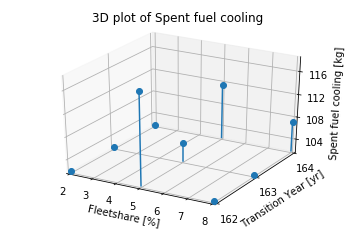
\includegraphics[width=0.4\linewidth]{figures/3d_sfc} 
        \caption{Inventory: Spent fuel cooling}
        \label{fig:3d_sfc}
    \end{subfigure}
    \begin{subfigure}[t]{0.4\textwidth}
        \centering
        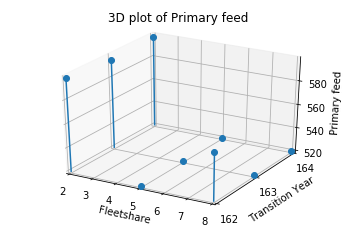
\includegraphics[width=\linewidth]{figures/3d_pf} 
        \caption{Inventory: Primary feed}
	    \label{fig:3d_pf}
    \end{subfigure}
    \begin{subfigure}[t]{0.4\textwidth}
        \centering
        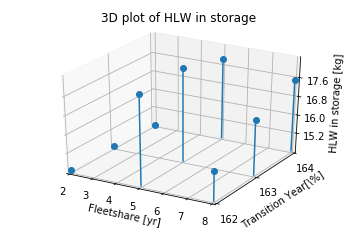
\includegraphics[width=\linewidth]{figures/3d_hlw} 
        \caption{Inventory: HLW in storage}
        \label{fig:3d_hlw}
    \end{subfigure}
    \caption{Maximum amount of Pu [kg] in each inventory during each simulation for varying fleet share and transition start date.}
\end{figure}

Figures \ref{fig:3d_sfc}, \ref{fig:3d_pf}, and \ref{fig:3d_hlw}
communicate how fleet share ratio and introduction date of advanced 
reactor technology 
synergistically impact maximum Pu in various inventories in the 
\gls{NFC}. 
To better utilize this information for decision making, 
similar synergistic studies can be conducted for the output 
variables in all the evaluation metrics. 
The results from each study can be normalized, weighted, and 
combined to create an optimization surface similar 
to \ref{fig:passerini_payoff} to determine the ideal fleet share 
ratio and transition year combination. 

\subsubsection{\textbf{Cyclus}}
25 scenarios were evaluated for a combination of fleet share ratio 
of 0\%, 5\%, 10\%, 15\%, 20\% PWR MOX and advanced reactor introduction 
date of year 80 to 84 years.
Figures \ref{fig:cyclus_3d_hlw}, \ref{fig:cyclus_3d_depu}, and \ref{fig:cyclus_3d_ic}
visualize the final amount of HLW, final amount of depleted uranium, and
total amount of idle capacity in the scenario for varying 
fleet share and advanced reactor introduction date values. 

Figure \ref{fig:cyclus_3d_hlw} shows that for scenarios in which 
there are less \gls{MOX} \glspl{PWR}, and when the transition begins 
later in the simulation, there is less high level waste produced. 
This is assuming that the initial \glspl{LWR} have a longer lifetime
and thus, less reprocessing waste is produced. 

Figure \ref{fig:cyclus_3d_depu} shows that as the introduction date 
of advanced reactors is pushed back, more depleted uranium is produced 
due to 

Figure \ref{fig:cyclus_3d_ic} shows that idle capacity is minimized 
for a later advanced reactor introduction date. 
Having a later introduction date of advanced reactor technology ensures 
that a sufficiently large inventory of transuranic elements is amassed
to produce fuel for the \gls{MOX} \glspl{PWR} and \glspl{SFR}.  
This ensures that there is no gap in the supply chain that results 
in idle advanced reactor capacity.

% replace transition year 
\begin{figure}[]
    \centering
    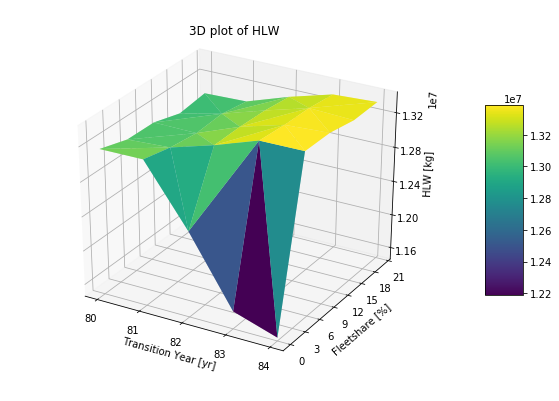
\includegraphics[width=0.7\linewidth]{cyclus_3d_hlw} 
    \caption{Final amount of HLW [kg] in the scenario during each simulation for varying fleet share and transition start date.}
    \label{fig:cyclus_3d_hlw}
\end{figure}

% replace transition year 
\begin{figure}[]
    \centering
    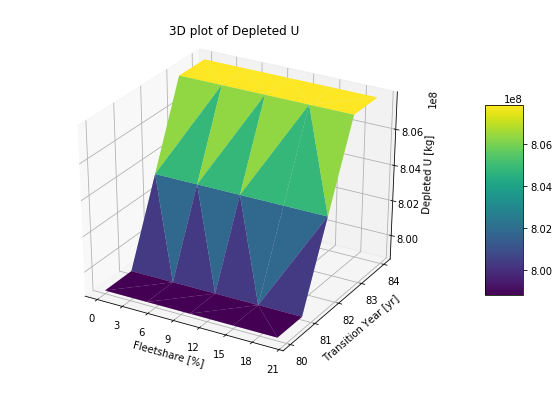
\includegraphics[width=0.7\linewidth]{cyclus_3d_depu} 
    \caption{Final amount of Depleted Uranium [kg] in the scenario during each simulation for varying fleet share and transition start date.}
    \label{fig:cyclus_3d_depu}
\end{figure}

% replace transition year 
\begin{figure}[]
    \centering
    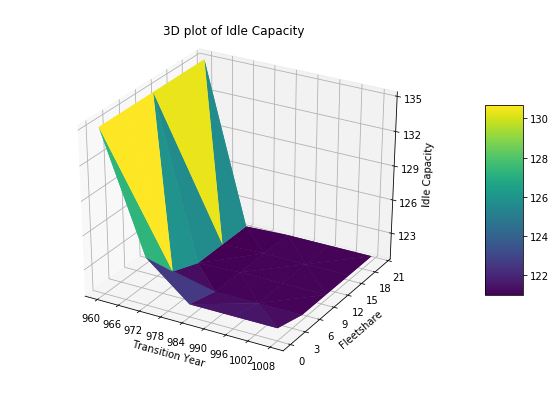
\includegraphics[width=0.7\linewidth]{cyclus_3d_ic} 
    \caption{Total amount of Idle Capacity [MW] in the scenario during each simulation for varying fleet share and transition start date.}
    \label{fig:cyclus_3d_ic}
\end{figure}

\section{Global Sensitivity Analysis}
\texttt{dcwrapper} was used to conduct a global sensitivity 
analysis study to generate Sobol indices' which tells us which 
input parameters has the most influence on an output variable. 
This type of sensitivity analysis was described in 
section \ref{sec:sobol}. 
It is more effective than OAT (section \ref{sec:oat}) and 
synergistic (section \ref{sec:synergistic}) sensitivity 
analysis, because it decomposes the variance of the 
output of the scenario simulation into fractions which can be 
attributed to each input, giving a better idea of the
most impactful input parameters. 
More than two variables could be varied in a synergistic
sensitivity analysis, but it is difficult to visualize the 
results. 

The input variables varied are: fleet share ratio, 
transition start year, and used fuel cooling time.
The output variables considered are final amount of HLW, 
final amount of depleted uranium, and total idle capacity. 
Table \ref{tab:sobol} shows the results of the study. 
